\documentclass[aps,twocolumn,secnumarabic,balancelastpage,amsmath,amssymb,nofootinbib,floatfix]{revtex4-1}

\usepackage{graphicx}      % tools for importing graphics
\usepackage[colorlinks=true]{hyperref}  % this package should be added 
\usepackage{dcolumn}% Align table columns on decimal point
\usepackage{bm}% bold math
\usepackage{xcolor}

\usepackage{tikz}         % tools for drawing figures
\setlength{\parskip}{5pt}
\usetikzlibrary{decorations.pathmorphing}

\newcommand{\kev}{\,{\rm keV}}
\newcommand{\s}{\,{\rm s}}


\begin{document}

\title{Compton scattering}

\author{Vinh Tran}
\affiliation{Department of Physics and Kavli Institute for Astrophysics and Space Research, Massachusetts Institute of Technology, Cambridge, MA 02139, USA}
\email{vinhtran@mit.edu}

\date{\today}

%%%%%%%%%%%%%%%%%%%%%%%%%%%%%%%%%%%%%%%%%%%%%%%%%%%%%%%%%%%%%%%%%%

\begin{abstract}



\end{abstract}

\maketitle

%%%%%%%%%%%%%%%%%%%%%%%%%%%%%%%%%%%%%%%%%%%%%%%%%%%%%%%%%%%%%%%%%%

\section{Introduction}
\label{sec:intro}




\section{Inelastic scattering of photon}
\label{sec:theory}

\subsection{Scattering kinematics}
\label{ssec:scattering_kinematics}

\begin{figure}[h]
    \centering
    \vspace{-0.75cm} % Adjust this value as needed to reduce extra space above the figure
    \begin{tikzpicture}[scale=1.5,>=stealth, baseline={(0,0)}]
        % Draw the incident photon arrow (from left to the vertex)
        \draw[decorate, decoration={snake, amplitude=0.5mm, segment length=4mm}, thick, ->] (-2,0) -- (0,0) node[midway, above, inner sep=5] {$\gamma$};
    
        \draw[-, dashed] (0,0) -- (2,0);
    
        % Mark the scattering vertex
        \fill (0,0) circle (1.5pt);
    
        % Draw the recoil electron arrow (at phi=30° above horizontal)
        \draw[->, thick](0,0) -- ({2*cos(-45)},{2*sin(-45)}) node[midway, below, inner sep=10] {$e^-$};
        
        % Draw the scattered photon arrow (at theta=20°)
        \draw[decorate, decoration={snake, amplitude=0.5mm, segment length=4mm}, thick, ->]  (0,0) -- ({2*cos(30)},{2*sin(30)}) node[midway, above, inner sep=10] {$\gamma'$};
    
        % Mark the recoil angle phi (single arc for clarity)
        \draw (0.375,0) arc (0:-45:0.375);
        \draw (0.425,0) arc (0:-45:0.425);
        \node at (0.6,-0.25) {$\phi$};
    
        % Mark the scattering angle theta (double arc from horizontal to electron arrow)
        \draw (0.4,0) arc (0:30:0.4);
        \node at (0.6,0.15) {$\theta$};
    \end{tikzpicture}
    \caption{Compton scattering of a photon by an electron. $\gamma$ and $\gamma'$ are the incident and scattered photons. $e^-$ is the recoil electron initially at rest. $\theta$ and $\phi$ are the scattering and recoil angles, respectively.}
    \label{fig:scattering}
\end{figure}

Following relativistic kinematics, we treat photons as massless particles of energy $E_\gamma = h \nu$, where $h$ is the Planck constant and $\nu$ is the photon frequency. The energy of an electron is given by $E_e = \sqrt{m_e^2 c^4 + p_e^2 c^2}$, where $m_e$ is the electron rest mass, $p_e$ is the electron momentum, and $c$ is the speed of light. By conservation of energy $E$ and momentum $\vec{p}$, we have
\begin{align}
    \label{eq:energy_conservation}
    E_\gamma + E_e &= E_\gamma^{\prime} + E_e^{\prime}, \\
    \label{eq:momentum_conservation}
    \vec{p}_\gamma + \vec{p}_e &= {\vec{p}_\gamma}^{\,\prime} + {\vec{p}_e}^{\,\prime},
\end{align}
where the prime denotes the final state. For simplicity, we take the initial electron energy as $E_e = m_e c^2$, that is the particle is initially at rest. Solving Equations \eqref{eq:energy_conservation} and \eqref{eq:momentum_conservation}, we obtain the energy of the scattered photon as
\begin{equation}
    \label{eq:scattered_photon_energy}
    E_\gamma^{\prime} = \frac{E_\gamma}{1 + \frac{E_\gamma}{m_e c^2} (1 - \cos \theta)},
\end{equation}
with $\theta$ being the scattering angle, i.e. the angle between the initial and final photon momenta. The kinetic energy of the recoil electron is then approximated as $E_e^{\prime} = E_\gamma - E_\gamma^{\prime}$. The scattering scheme is illustrated in Figure \ref{fig:scattering}.


\subsection{Differential cross section}
\label{ssec:differential_cross_section}

In the classical regime, the cross section of Compton scattering can be approximated by the Thomson formula for elastic collisions~\citep{Jackson1975}, given by
\begin{equation}
    \label{eq:thomson_cross_section}
    \frac{d\sigma}{d\Omega} = \left( \frac{e^2}{4 \pi \epsilon_0 m_e c^2} \right) \frac{1 + \cos^2{\theta}}{2},
\end{equation}
with $e$ being the electron charge and $\epsilon_0$ the vacuum permittivity.


\section{Experiment setup}
\label{sec:experiment}

\subsection{Apparatus}
\label{ssec:apparatus}

\subsection{Data collection}
\label{ssec:data_collection}

\begin{table}
    \centering
    \addtolength{\tabcolsep}{3pt}
    \def\arraystretch{1.2}
    \begin{tabular}{c c c c}
        \hline
        $\theta$ & Counting Time & Total Time & Collection Date \\ [0ex]
        $[\rm{deg}]$ & $[\rm{s}]$ & $[\rm{s}]$ & [YYYY-MM-DD] \\ [1ex]
        \hline\hline

        0 & 964 & 1012 & 2025-03-04 \\
        30 & 1194 & 1224 & 2025-03-04 \\
        60 & 1619 & 1658 & 2025-03-04 \\
        90 & 1856 & 1900 & 2025-03-04 \\
        120 & 1706 & 1736 & 2025-03-04 \\
        15 & 1354 & 1522 & 2025-03-06 \\
        45 & 1333 & 1455 & 2025-03-06 \\
        75 & 1954 & 2058 & 2025-03-06 \\
        105 & 1645 & 1727 & 2025-03-06 \\
        135 & 1341 & 1431 & 2025-03-06 \\
        
        \hline
        
    \end{tabular}
    \caption{}
    \label{tab:data_collection}    
\end{table}

\subsection{MCA calibration}
\label{ssec:calibration}

\begin{figure}
    \centering
    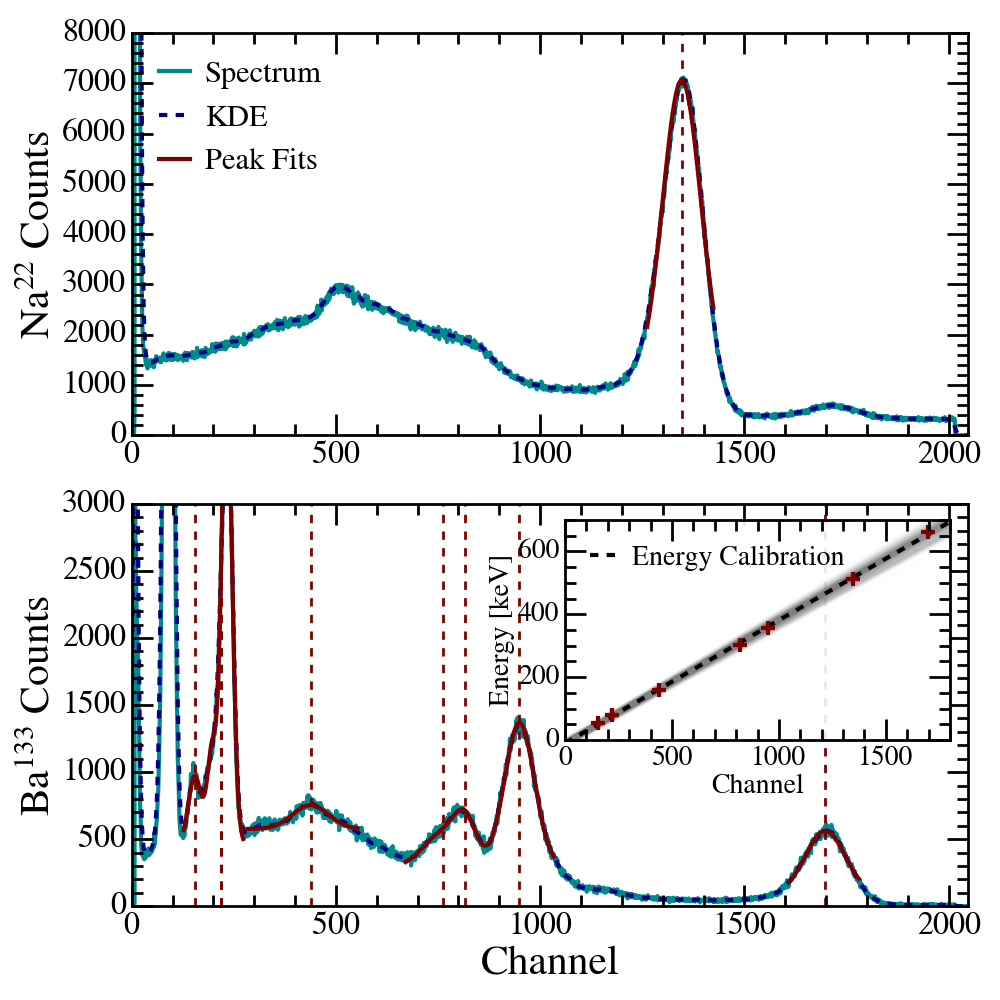
\includegraphics[width=0.49 \textwidth]{Figures/energy_calibration.png}
    \caption{}
    \label{fig:energy_calibration}
\end{figure}


\section{Results}
\label{sec:result}

\subsection{Energy-angle dependency}
\label{ssec:energy_angle_dependency}

\begin{figure}
    \centering
    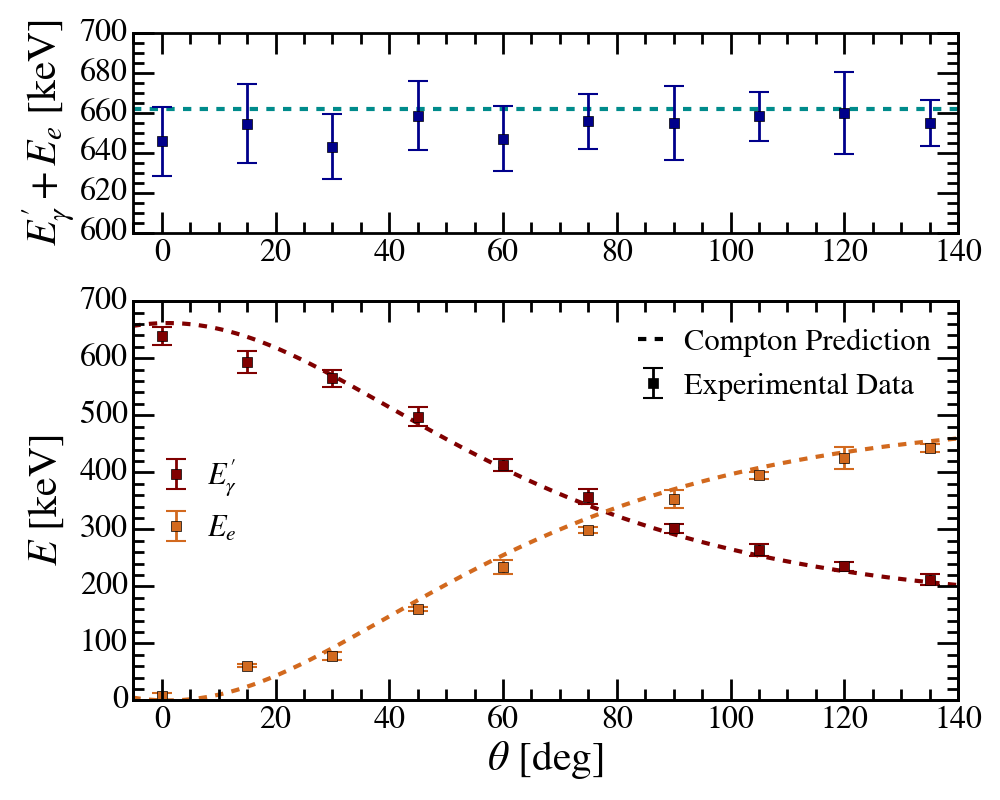
\includegraphics[width=0.49 \textwidth]{Figures/energy_angle_dependency.png}
    \caption{}
    \label{fig:energy_angle_dependency}
\end{figure}

\subsection{Scattering rate}
\label{ssec:scattering_rate}

\begin{figure}
    \centering
    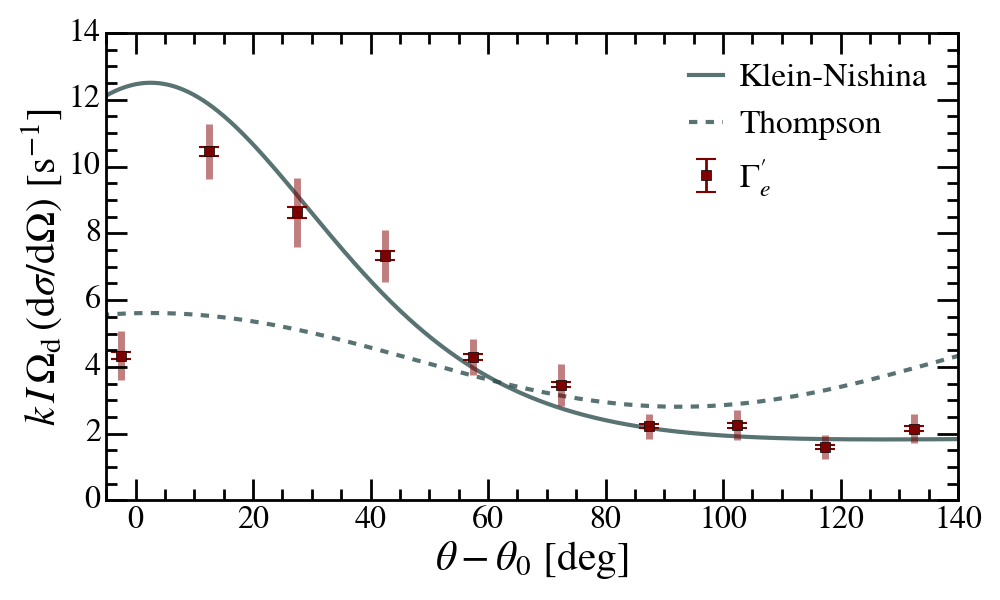
\includegraphics[width=0.49 \textwidth]{Figures/scattering_rate.png}
    \caption{}
    \label{fig:scattering_rate}
\end{figure}




\section{Discussion \& conclusion}
\label{sec:conclusion}




\begin{acknowledgments}

The author thanks his lab partner  Y. Hu for collaboration in the experiment, support in the formatting and structuring of the manuscript. The author also thanks the JLab teaching staffs for their guidance and support, as well as the MIT Physics Department for providing the experimental apparatus.

\end{acknowledgments}

%%%%%%%%%%%%%%%%%%%%%%%%%%%%%%%%%%%%%%%%%%%%%%%%%%%%%%%%%%%%%%%%%%

\bibliography{ref}

%%%%%%%%%%%%%%%%%%%%%%%%%%%%%%%%%%%%%%%%%%%%%%%%%%%%%%%%%%%%%%%%%%

\appendix